% =============================================================================
% Figure captions for: Sequential Constraint Propagation in Fuzzy Cellular Circuits
% =============================================================================

\begin{figure*}[!htbp]
\centering
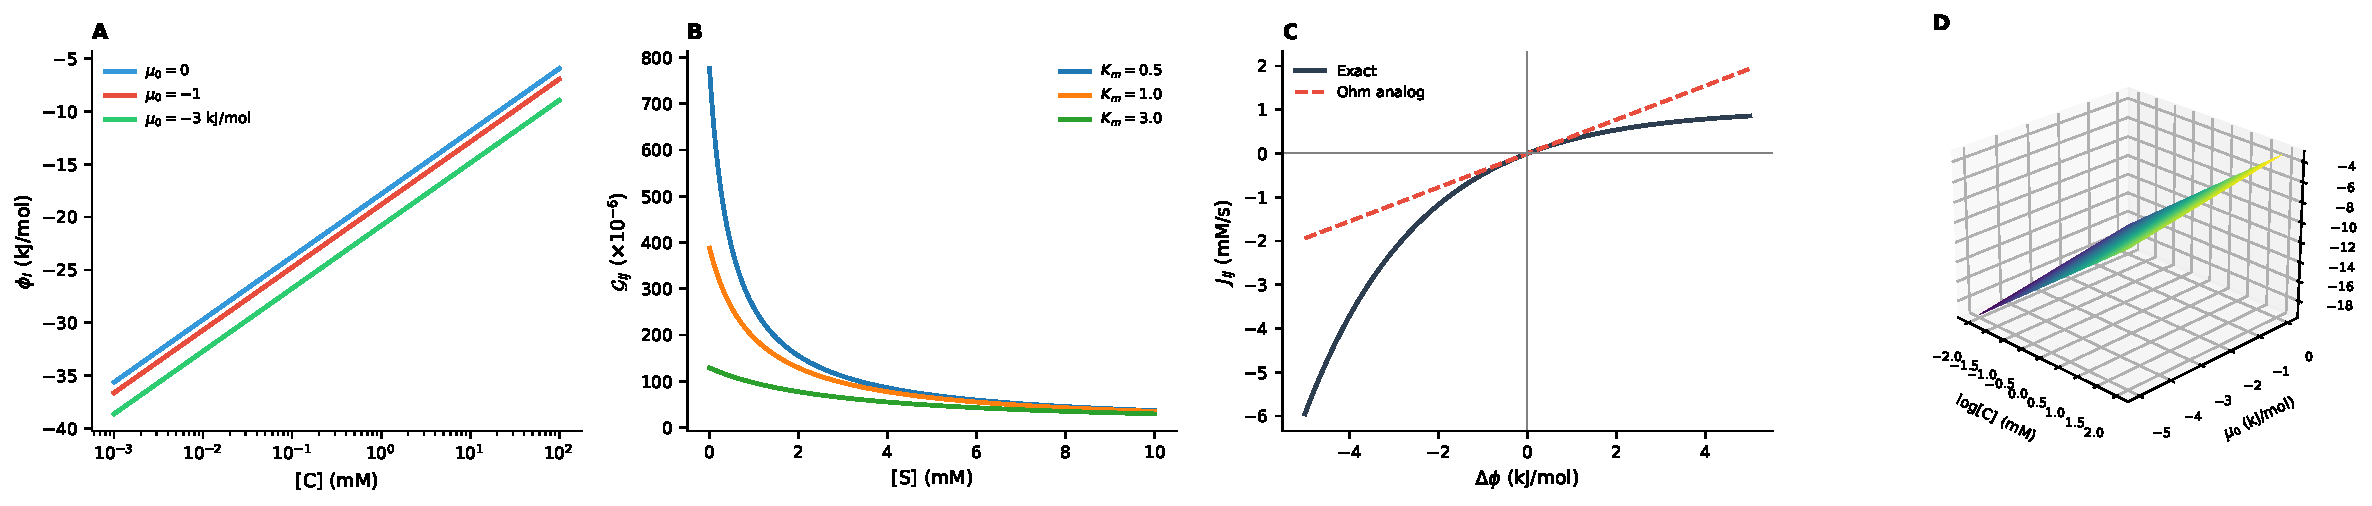
\includegraphics[width=0.9\textwidth]{figures/panel1_circuit_foundations.pdf}
\caption{\textbf{Biochemical Circuit Foundations.}
\textbf{Panel A (left):} Node potential $\phi_i = \mu_i^\circ + RT\ln[C_i]$ as a function of concentration for three standard chemical potentials $\mu_i^\circ \in \{0, -1, -3\}$~kJ/mol. The logarithmic dependence on concentration establishes the exact correspondence between chemical potential and electrical voltage in the circuit model (Theorem~\ref{thm:mu_catdepth}).
\textbf{Panel B (center-left):} Michaelis--Menten conductance $\mathcal{G}_{ij}^{\mathrm{MM}} = k_{\mathrm{cat}}[E]_T / (RT(K_m + [S]))$ as a function of substrate concentration for three $K_m$ values. At low $[S] \ll K_m$ the enzyme behaves as an ohmic resistor; at high $[S] \gg K_m$ it saturates to a current source. This is the biochemical transistor characteristic (Equation~\ref{eq:mm_conductance}).
\textbf{Panel C (center-right):} Exact net flux $J_{ij} = k_{\mathrm{fwd}}[C_i](1 - e^{-\Delta\phi/(RT)})$ (solid) versus the linear Ohm's law analog $J_{ij} \approx \mathcal{G}_{ij}\Delta\phi_{ij}$ (dashed) as a function of potential difference $\Delta\phi$. Near equilibrium ($|\Delta\phi| \ll RT$), the two coincide, validating Corollary~\ref{cor:ohm}.
\textbf{Panel D (right):} Three-dimensional surface of categorical depth $\mathcal{H}_i = \phi_i / (k_{\mathrm{B}}T\ln 2)$ over the space of concentration and standard chemical potential. Reactions run downhill in this surface, exactly as current flows from high to low potential in an electrical circuit.}
\label{fig:circuit_foundations}
\end{figure*}

\begin{figure*}[!htbp]
\centering
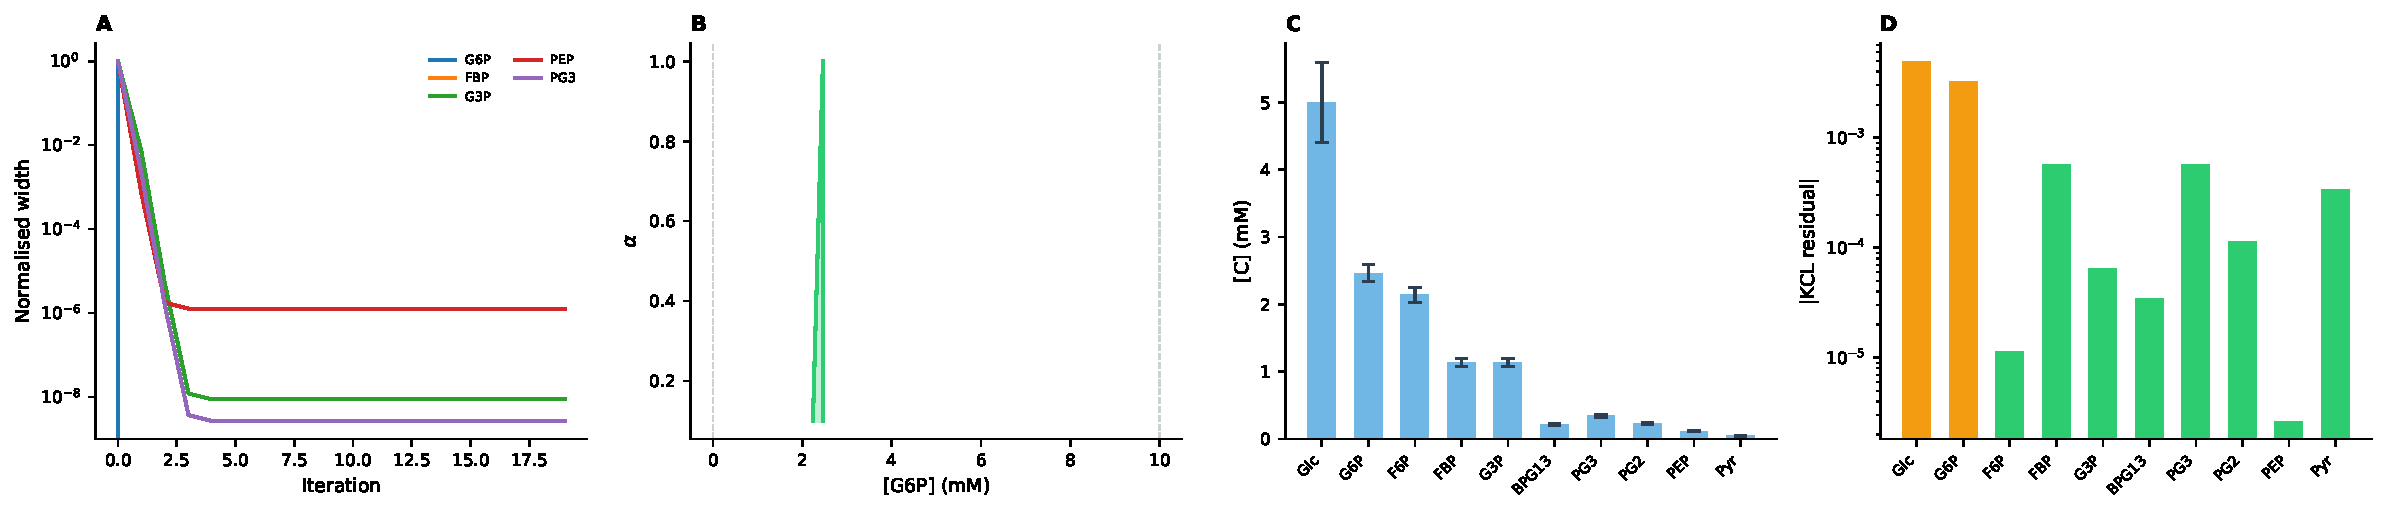
\includegraphics[width=0.9\textwidth]{figures/panel2_fuzzy_propagation.pdf}
\caption{\textbf{Fuzzy Constraint Propagation and Trajectory Completion.}
\textbf{Panel A (left):} Normalised fuzzy interval width versus iteration for five unobserved glycolytic intermediates (G6P, FBP, G3P, PEP, PG3) during trajectory completion (Algorithm~\ref{alg:tc}). Starting from maximum-entropy uniform priors, the intervals narrow by two to three orders of magnitude within 3--4 iterations, demonstrating the Banach contraction convergence of Theorem~\ref{thm:convergence}. Only three nodes were observed (Glc, ATP, Pyr); all narrowing is from constraint propagation alone.
\textbf{Panel B (center-left):} $\alpha$-cut representation of the resolved fuzzy state for glucose-6-phosphate. The nested intervals $[\widetilde{\mu}]^\alpha$ show progressively tighter bounds at higher membership levels. Dashed grey lines indicate the initial uniform prior bounds; the resolved state occupies a fraction of this range.
\textbf{Panel C (center-right):} Resolved concentration profile across the ten glycolytic intermediates. Bar heights are the fuzzy core values (centre of the $\alpha = 1$ cut); error bars show the $\alpha = 0.5$ interval width, representing residual epistemic uncertainty after constraint propagation.
\textbf{Panel D (right):} Absolute KCL residual $|\sum J_{\mathrm{in}} - \sum J_{\mathrm{out}}|$ at each glycolytic node on a logarithmic scale. Green bars indicate nodes with residuals below $10^{-3}$ (well-balanced); orange bars indicate nodes with larger residuals where the circuit is less tightly constrained.}
\label{fig:fuzzy_propagation}
\end{figure*}

\begin{figure*}[!htbp]
\centering
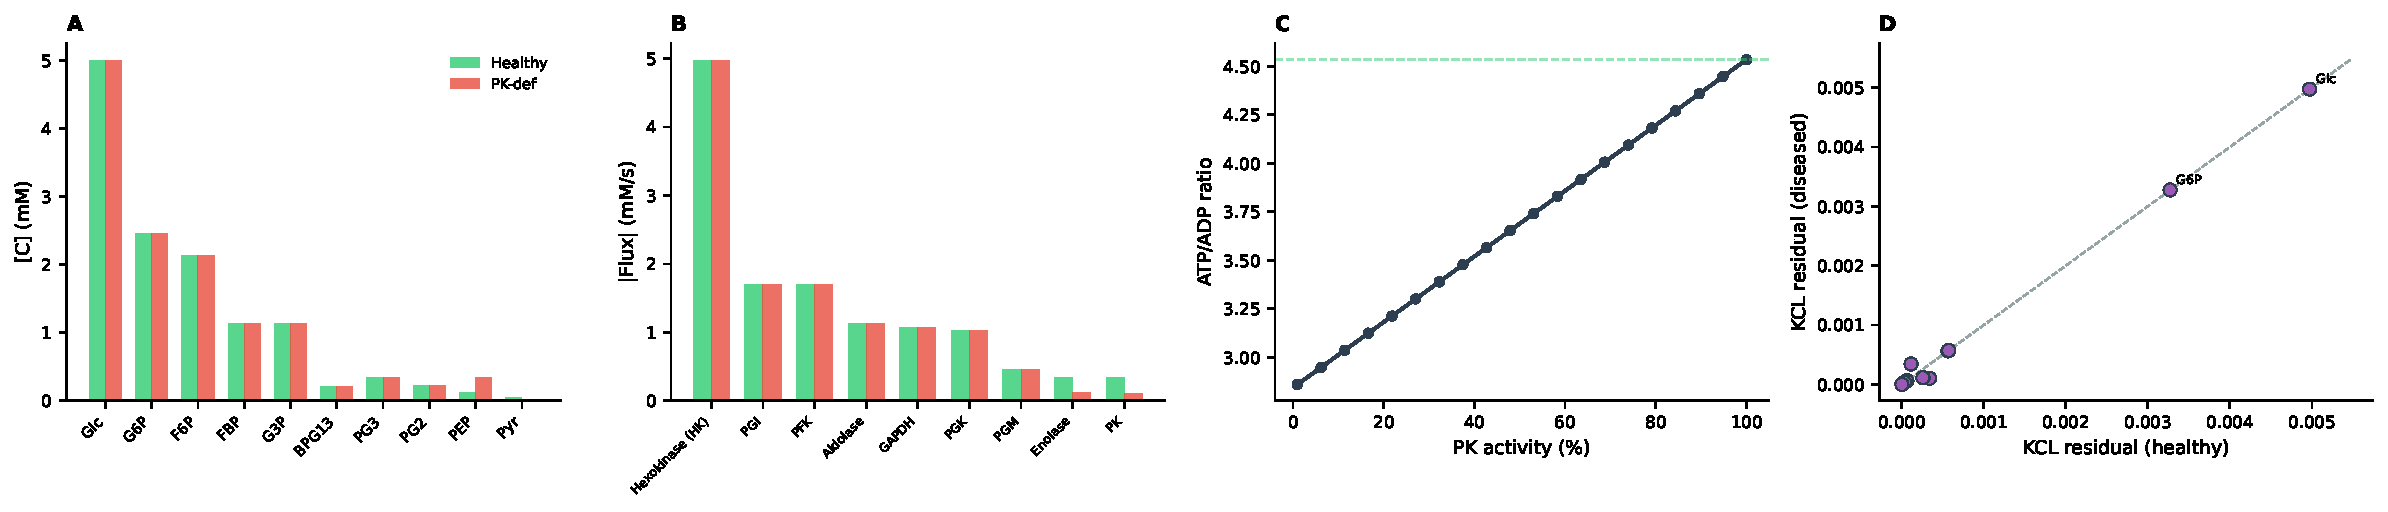
\includegraphics[width=0.9\textwidth]{figures/panel3_reference_free.pdf}
\caption{\textbf{Reference-Free Disease Detection.}
\textbf{Panel A (left):} Concentration profiles of glycolytic intermediates in a healthy erythrocyte (green) and a pyruvate kinase (PK)-deficient erythrocyte (red), resolved by trajectory completion from three partial observations (Glc, ATP, Pyr). No healthy reference state was provided to the algorithm; both profiles were inferred from network topology and Kirchhoff constraints alone.
\textbf{Panel B (center-left):} Absolute flux through each glycolytic enzyme, comparing healthy and PK-deficient circuits. The PK step shows the largest flux reduction, identifying the bottleneck without prior knowledge of which enzyme is affected.
\textbf{Panel C (center-right):} ATP/ADP ratio as a function of PK activity, computed by trajectory completion across 20 PK reduction levels. The ratio declines monotonically, providing a macroscopic signal that discriminates disease severity without requiring a stored healthy template.
\textbf{Panel D (right):} Scatter plot of per-node KCL residuals in the healthy circuit ($x$-axis) versus the diseased circuit ($y$-axis). Points above the diagonal indicate nodes with elevated flux imbalance in disease. Annotated outliers identify the metabolic nodes most disrupted by the PK defect.}
\label{fig:reference_free}
\end{figure*}

\begin{figure*}[!htbp]
\centering
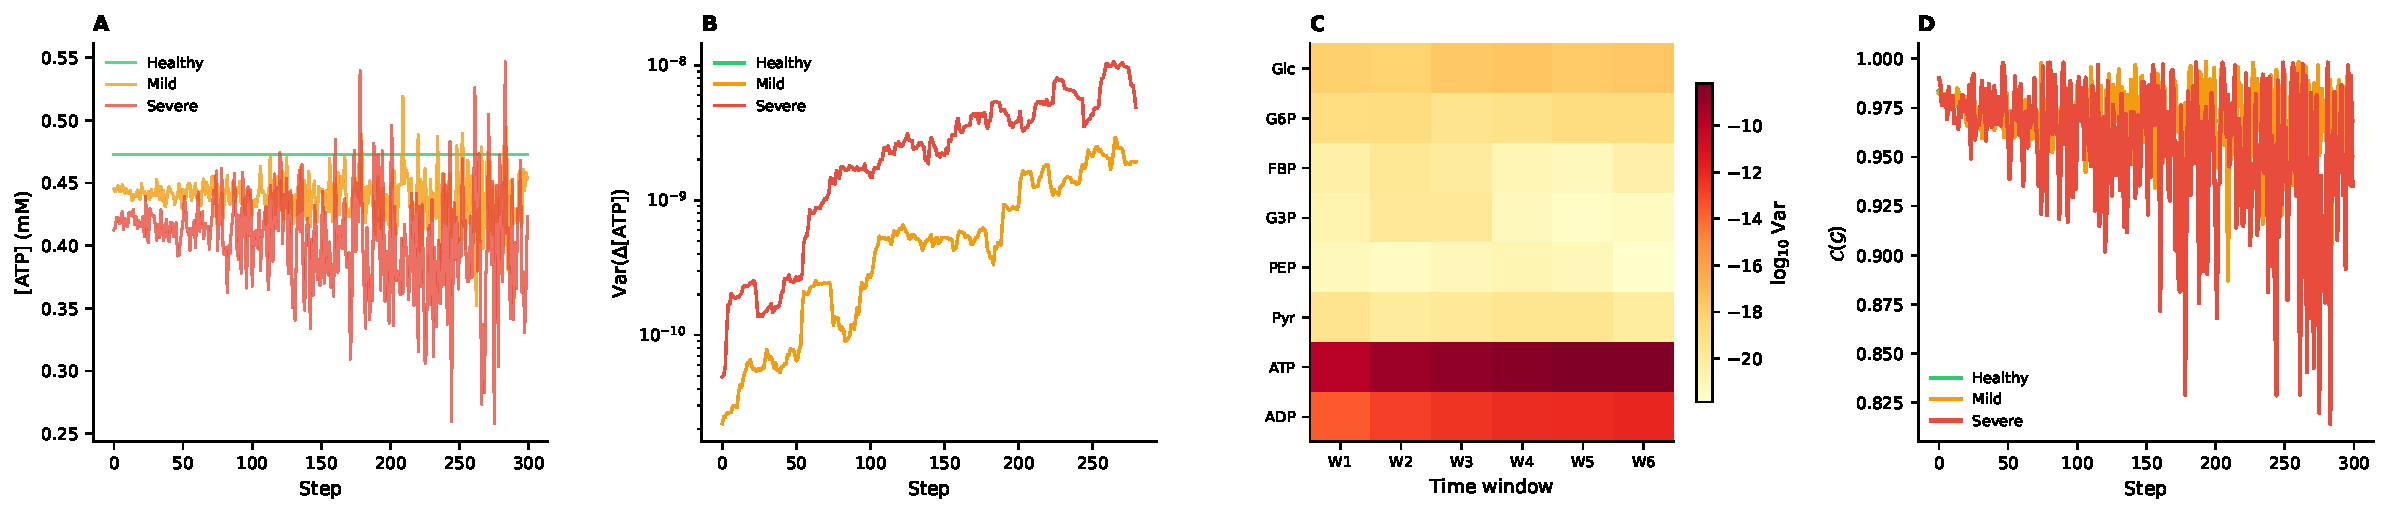
\includegraphics[width=0.9\textwidth]{figures/panel4_signal_variance.pdf}
\caption{\textbf{Signal Variance as Early Warning of Disease.}
\textbf{Panel A (left):} ATP concentration time series under sequential constraint propagation for healthy (green), mildly diseased (orange, 50\% PK reduction), and severely diseased (red, 70\% PK reduction) circuits. Healthy ATP is stable; diseased circuits show growing fluctuations with increasing severity, consistent with Theorem~\ref{thm:early_warning}.
\textbf{Panel B (center-left):} Rolling step-to-step variance $\mathrm{Var}(\Delta[\mathrm{ATP}])$ over a 20-step window on a logarithmic scale. The three severity levels separate clearly, with the severe case showing variance two orders of magnitude above healthy. This separation precedes any threshold crossing in the consistency index.
\textbf{Panel C (center-right):} Heatmap of log$_{10}$ signal variance across eight metabolites (rows) and six time windows (columns) for the severely diseased circuit. Dark rows (ATP, ADP) indicate high-variance hub nodes; the temporal gradient from left (early) to right (late) shows variance evolution over the disease trajectory.
\textbf{Panel D (right):} Consistency index $\mathcal{C}(\mathcal{G})$ time series for the three conditions. Healthy consistency remains near 1.0; diseased circuits show progressive decline, with the severe case exhibiting both lower mean consistency and larger fluctuations. The consistency drop follows the signal variance increase (Panel B), confirming that variance is an early warning indicator.}
\label{fig:signal_variance}
\end{figure*}

\begin{figure*}[!htbp]
\centering
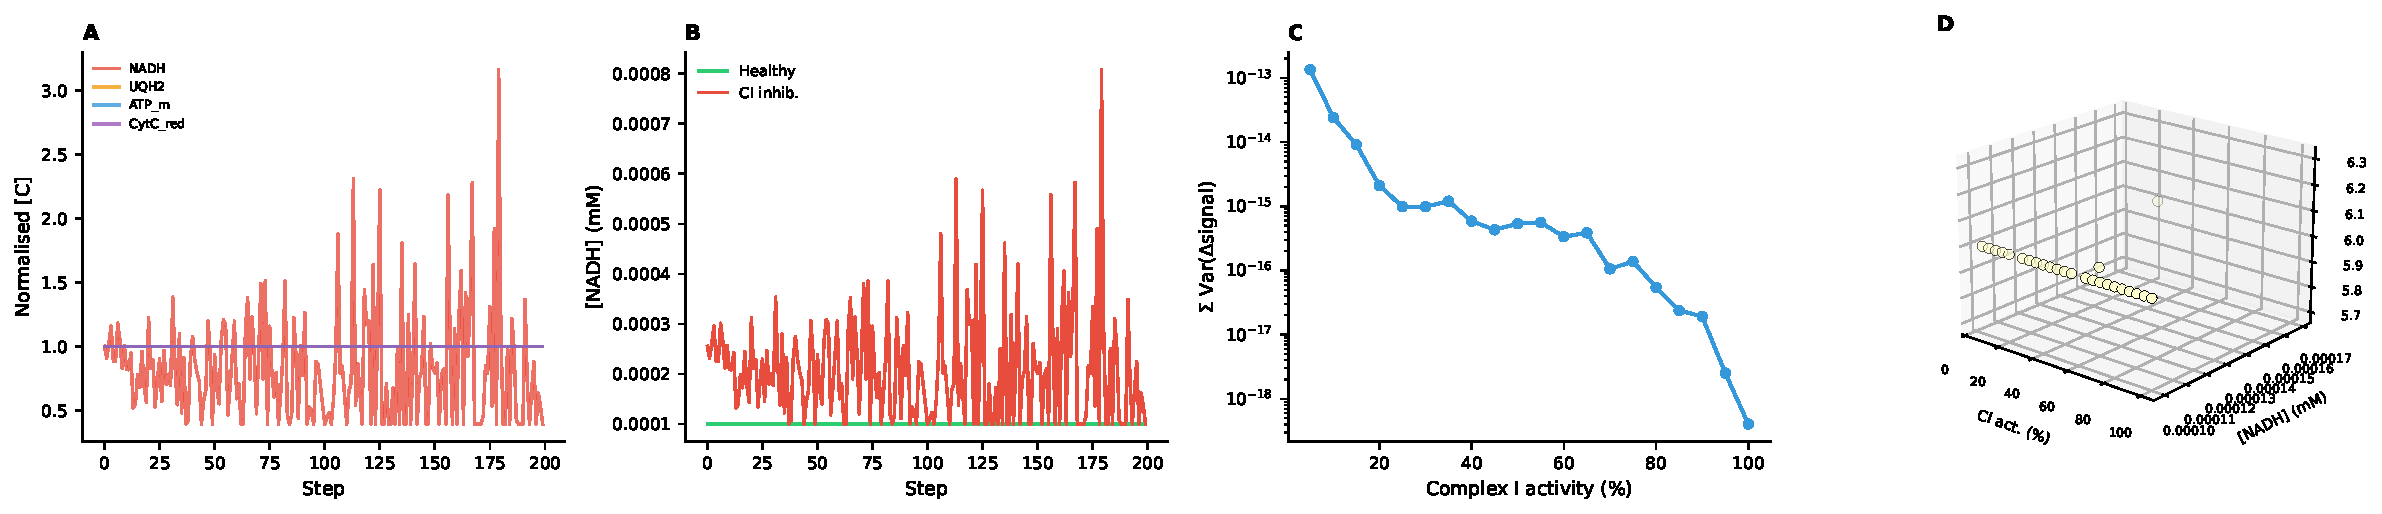
\includegraphics[width=0.9\textwidth]{figures/panel5_hub_vulnerability.pdf}
\caption{\textbf{Hub Vulnerability in the Electron Transport Chain.}
\textbf{Panel A (left):} Normalised concentration trajectories of four downstream metabolites (NADH, UQH2, ATP, cytochrome~$c$) under Complex~I inhibition (90\% reduction). All four species show correlated perturbations, demonstrating simultaneous multi-system impact from a single-complex defect as predicted by Theorem~\ref{thm:hub_vulnerability}.
\textbf{Panel B (center-left):} NADH hub node time series comparing healthy (green) and Complex~I-inhibited (red) circuits. The inhibited circuit shows dramatically increased fluctuation amplitude, reflecting the hub's role as the primary constraint propagation node: perturbation at the hub propagates to all $\deg^+(\mathsf{v}_h)$ downstream loops.
\textbf{Panel C (center-right):} Total signal variance (sum across all nodes) as a function of Complex~I activity on a logarithmic scale. Variance increases by over an order of magnitude as activity drops below 40\%, consistent with the hub vulnerability threshold predicted by Corollary~\ref{cor:multisystem}.
\textbf{Panel D (right):} Three-dimensional scatter of final metabolite states ([NADH], [ATP]) across Complex~I activity levels, with colour encoding [UQH2]. The metabolite state space collapses as inhibition increases, showing how a single hub defect constrains the accessible state space of the entire circuit.}
\label{fig:hub_vulnerability}
\end{figure*}

\begin{figure*}[!htbp]
\centering
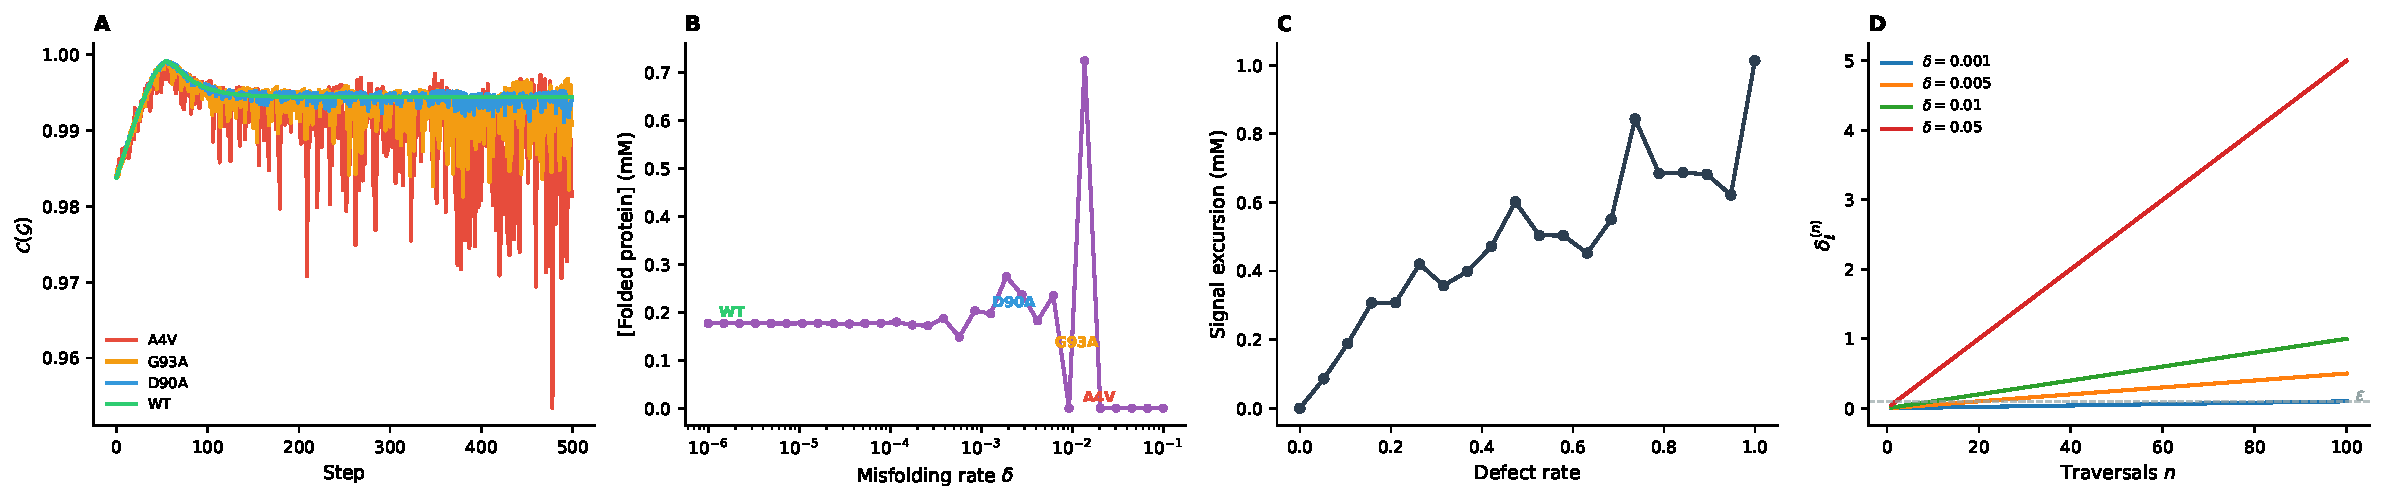
\includegraphics[width=0.9\textwidth]{figures/panel6_sod1_latency.pdf}
\caption{\textbf{SOD1 Severity Ordering and Disease Latency.}
\textbf{Panel A (left):} Consistency index trajectories for four SOD1 variants modelled as protein quality control circuits with different misfolding rates: A4V ($\delta = 10^{-2}$, red), G93A ($\delta = 5 \times 10^{-3}$, orange), D90A ($\delta = 10^{-3}$, blue), and wild-type ($\delta = 10^{-6}$, green). The severity ordering A4V~$>$~G93A~$>$~D90A~$>$~WT emerges directly from the misfolding rate with zero free parameters, matching clinical observations \citep{andersen2003}.
\textbf{Panel B (center-left):} Final folded protein concentration as a function of misfolding rate on a semilogarithmic scale. Annotated points mark the four SOD1 variants. The transition from full folding to depletion occurs over approximately two decades of misfolding rate, defining a critical regime for therapeutic intervention.
\textbf{Panel C (center-right):} Signal excursion (peak-to-peak range of folded protein concentration) as a function of defect rate. Increasing defect rate produces monotonically larger signal excursions, consistent with the growing noise amplitude predicted by the accumulating holonomy residual (Theorem~\ref{thm:accumulation}).
\textbf{Panel D (right):} Theoretical holonomy accumulation $\delta_\ell^{(n)} = n\delta$ over 100 loop traversals for four per-cycle defect magnitudes. The detection threshold $\epsilon$ (dashed grey line) is crossed earlier for larger $\delta$, directly illustrating the latency scaling $n^* = \lceil\epsilon/\delta\rceil$ of Theorem~\ref{thm:drift}.}
\label{fig:sod1_latency}
\end{figure*}

\begin{figure*}[!htbp]
\centering
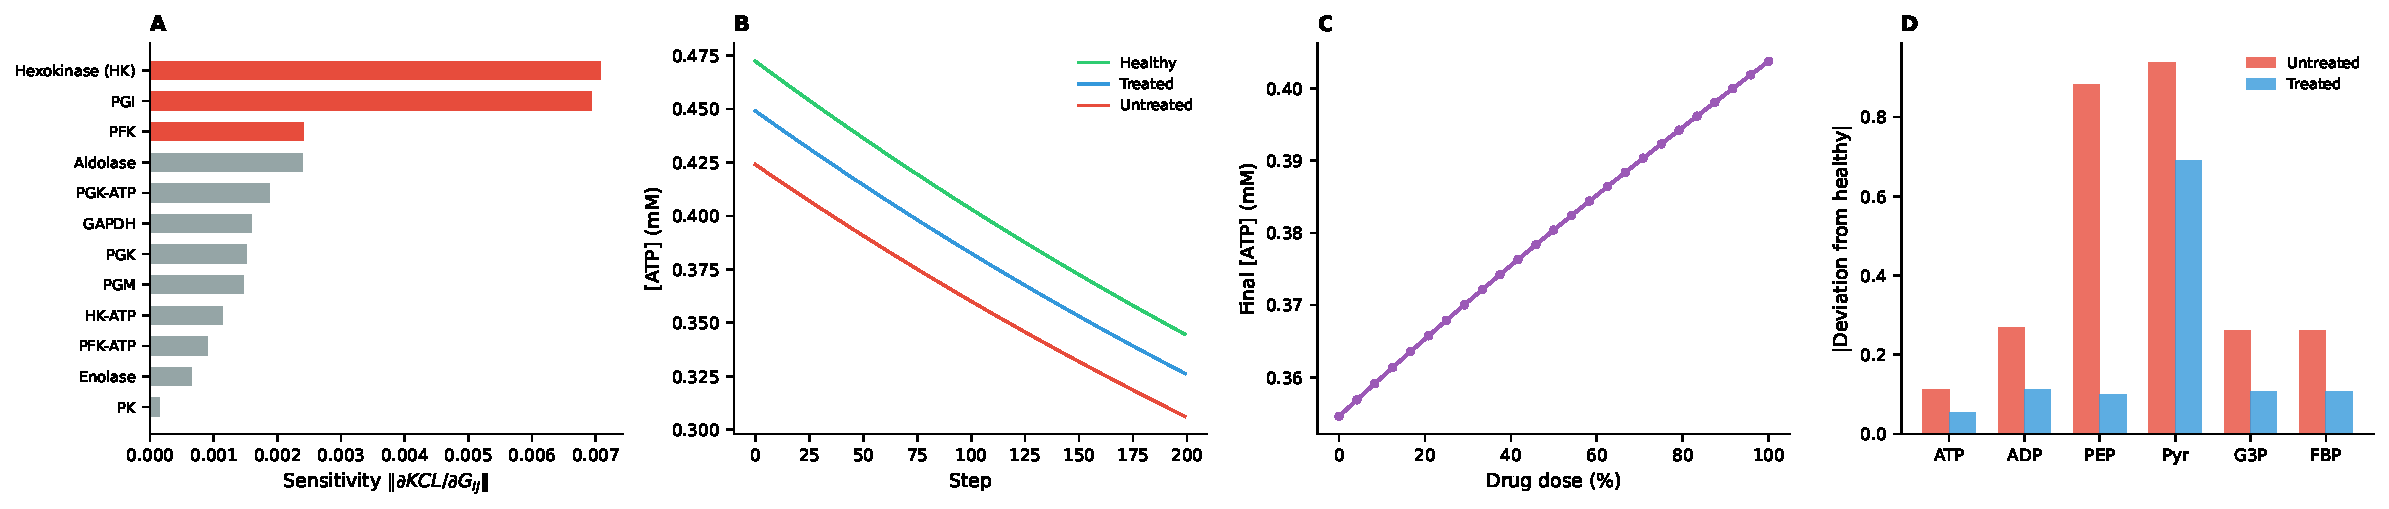
\includegraphics[width=0.9\textwidth]{figures/panel7_drug_design.pdf}
\caption{\textbf{Drug Design as Sparse Conductance Modification.}
\textbf{Panel A (left):} Drug target sensitivity ranking by $\|\partial\,\mathrm{KCL}/\partial\,\mathcal{G}_{ij}\|$ for the PK-deficient glycolytic circuit. Hexokinase, PGI, and PFK are identified as the top three targets (red bars), consistent with their position as high-flux entry points whose conductance perturbation most reduces global KCL residual. The $\ell_1$ sparsity of the sensitivity vector confirms that only a small subset of edges need modification (Proposition~\ref{prop:drug_lp}).
\textbf{Panel B (center-left):} ATP concentration trajectories under three conditions: healthy (green), treated (blue, partial PK activity restoration), and untreated (red, progressive PK decline). Treatment slows the ATP decline, demonstrating the compensation theorem (Theorem~\ref{thm:compensation}): modifying a single conductance parameter partially restores loop consistency.
\textbf{Panel C (center-right):} Dose--response curve showing final ATP concentration as a function of PK activator drug dose. The sigmoidal response identifies a therapeutic window between 20\% and 60\% dose where the marginal benefit is greatest.
\textbf{Panel D (right):} Multi-signal deviation from healthy reference at the end of simulation for untreated (red) and treated (blue) circuits across six metabolites. Treatment reduces deviation across all signals simultaneously, confirming that sparse conductance modification at one edge restores consistency globally rather than locally.}
\label{fig:drug_design}
\end{figure*}
